\documentclass[11pt]{article}


\usepackage{fullpage}
\usepackage{graphicx}
\usepackage{amsmath}
\usepackage{amssymb}
\usepackage{amsthm}
\usepackage{fancyvrb}

\newcommand{\myname}{Mehshan Mustafa}

\newenvironment{theorem}[2][Theorem]{\begin{trivlist}
\item[\hskip \labelsep {\bfseries #1}\hskip \labelsep {\bfseries #2.}]}{\end{trivlist}}
\newenvironment{lemma}[2][Lemma]{\begin{trivlist}
\item[\hskip \labelsep {\bfseries #1}\hskip \labelsep {\bfseries #2.}]}{\end{trivlist}}
\newenvironment{exercise}[2][Exercise]{\begin{trivlist}
\item[\hskip \labelsep {\bfseries #1}\hskip \labelsep {\bfseries #2.}]}{\end{trivlist}}
\newenvironment{problem}[2][Problem]{\begin{trivlist}
\item[\hskip \labelsep {\bfseries #1}\hskip \labelsep {\bfseries #2.}]}{\end{trivlist}}
\newenvironment{question}[2][Question]{\begin{trivlist}
\item[\hskip \labelsep {\bfseries #1}\hskip \labelsep {\bfseries #2.}]}{\end{trivlist}}
\newenvironment{corollary}[2][Corollary]{\begin{trivlist}
\item[\hskip \labelsep {\bfseries #1}\hskip \labelsep {\bfseries #2.}]}{\end{trivlist}}
\newenvironment{solution}{\begin{proof}[Solution]}{\end{proof}}
\newenvironment{idea}[2][Proof Idea.]{\textit{#1} #2}



\parindent0in
\pagestyle{plain}
\thispagestyle{plain}

\newcommand{\dated}{\today}
\newcommand{\token}[1]{\langle \text{#1} \rangle}

\begin{document}

\textbf{Introduction to the Theory of
Computation}\hfill\textbf{\myname}\\[0.01in]
\textbf{Chapter 3: The Church-Turing Thesis}\hfill\textbf{\dated}\\
\smallskip\hrule\bigskip

\begin{problem}{3.12}
A \textbf{\textit{Turing machine with left reset}} is similar to an ordinary Turing machine, but the transition function has the form
\[
\delta : Q \times \Gamma \longrightarrow Q \times \Gamma \times \{\text{R, RESET}\}.
\]

If $\delta(q, a) = (r, b, \text{RESET})$, when the machine is in state $q$ reading an $a$, the machine’s head jumps to the left-hand end of the tape after it writes $b$ on the tape and enters state $r$. Note that these machines do not have the usual ability to move the head one symbol left. Show that Turing machines with left reset recognize the class of Turing-recognizable languages.
\end{problem}

\begin{idea}[Informal description.]
We show how to simulate move left using move right and reset. Define \textit{target cell} as the cell, which is on the left of the current head position. If the head is positioned at either the first or second cell, then simply reset to move the head on the target cell. Otherwise, mark the current cell, reset to the start of the tape, and check one by one which cell is on the left of the target cell. Once it is found, reset and bring the head back on it and move right to position the head at the target cell.
\begin{center}
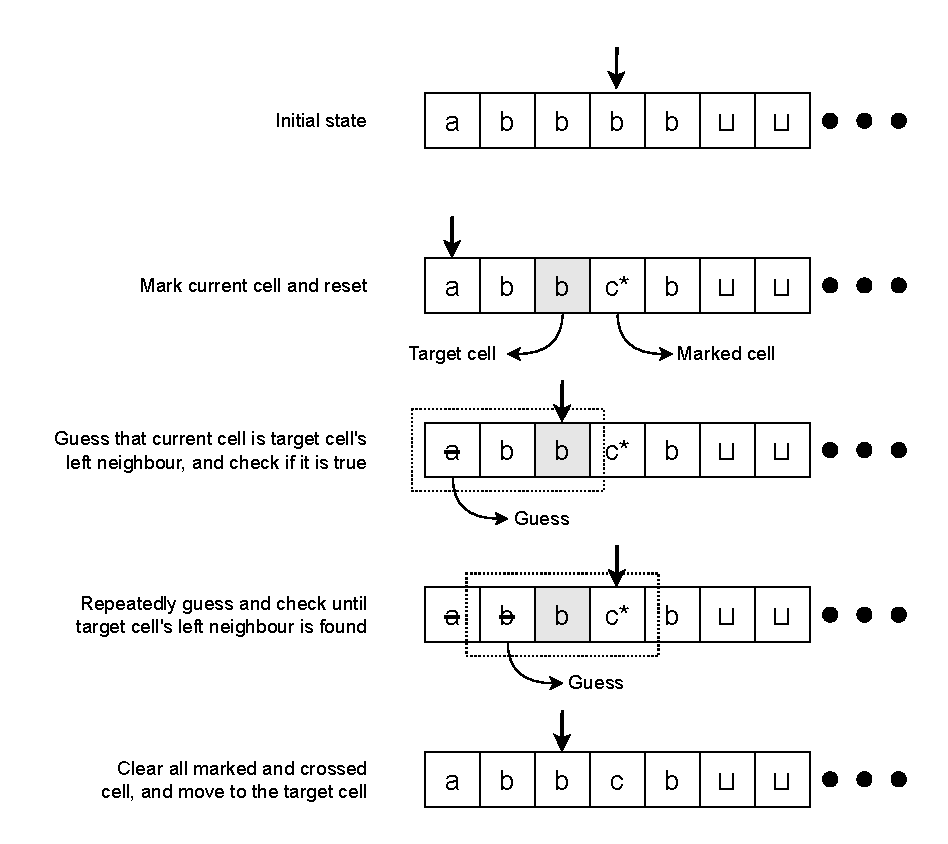
\includegraphics[scale=0.85]{Figures/Problem3.12.pdf} \\
Simulation of a left move.
\end{center}
\end{idea}

\begin{proof}
To show that Turing machines with left reset recognize the class of Turing-recognizable languages, we show how to simulate a move left in such machines.
\begin{enumerate}
\item Write the new symbol at the current head position with a mark and reset.
\item  If the symbol on the first or second position is marked, then it is the case of move left from first or second cell position. Simply, clear the mark and rest to simulate a move left. Otherwise, reset and go to stage 3.
\item Guess that current cell is on left of the target cell by crossing the symbol and move right.
\item Skip the cell and move right.
\item If the symbol at the current head position is marked, then clear the mark and reset. Next, repeatedly move right and clear crossed symbols until an uncrossed cell is reached, which is the target cell.
\item If the symbol at the current head position is unmarked, then rest. Repeatedly move right, skipping all crossed symbols until an uncrossed cell is reached, and then go to stage 3.
\end{enumerate}
\end{proof}

\end{document}
